\section{Regisztráció}


A regisztráció során biztosítanunk kell szerepköröket ${Sz}_{sz\acute{a}m}$, amivel kategorizálni tudjuk a felhasználókat. A felhasználóknak két csoportját különböztetjük meg: szakemberek és ügyfelek. Ezeket a kategóriákat egy felhasználó egyszerre is felveheti, ekkor külön nézet választóra lesz szükség. További szerepkör az adminisztrátor (oldal üzemeltetés), akinek validálnia kell a kivitelező által beállított kompetenciák hitelességét.

\subsection{Szerepkörök:}

\begin{itemize}
    \item ${Sz}_1$: Szakember
    \item ${Sz}_2$: Ügyfél
    \item ${Sz}_3$: Adminisztrátor
\end{itemize}

A szükséges adatok ${SA}_{sz\acute{a}m}$ megadásakor minden felhasználónak kötelező a név és életkor kitöltése. Szakembereknél mindenképpen megadásra kell kerülnie a kompetenciáknak, végzettségnek, ezeket előre megadott listából tudják kiválasztani. A munkatapasztalat megadásánál is vannak kötelező adatok: a munkával töltött évek száma, és a munkáihoz tartozó referencia, amelynek visszakövethetőnek kell lennie, ezt szintén ellenőrzésre fog kerülni az adminisztrátor által. Majd egy szerződés, amellyel biztosításra kerül a fizetési kötelezettség. Opcionálisan megadható lesz a szakembernek földrajzi helyzetének adatai.

\subsection{Szükséges adatok:}

\begin{itemize}
    \item Mindenkinek:
    \begin{itemize}
        \item ${SA}_1$: Név
        \item ${SA}_2$: Életkor
    \end{itemize}
    \item Szakembereknek:
    \begin{itemize}
        \item ${SA}_3$: Kompetencia
        \item ${SA}_4$: Végzettség
        \item ${SA}_5$: Munkatapasztalat
        \begin{itemize}
            \item ${SA}_{5.1}$: Évek száma
            \item ${SA}_{5.1}$: Referencia
        \end{itemize}
    \end{itemize}
    
    \item Megadható:
    \begin{itemize}
        \item ${SA}_6$: Földrajzi helyzet
    \end{itemize}
\end{itemize}

A regisztrációnál egyedi felhasználó nevet, illetve egy megfelelő erősségű jelszót kell megadnia az új felhasználónak, ami alapján egyrtelműen azonosítani lehet, illetve biztonságosan be tud lépni a fiókjába.

\subsection{Jelszó kritériumai:}

\begin{itemize}
    \item $J_1$: legalább 8 karakter
    \item $J_2$: legalább 1 számot kell tartalmaznia
    \item $J_3$: legalább 1 speciális karakternek kell benne szerepelnie
    \item $J_4$: legalább 1 nagy és 1 kisbetűt kell tartalmaznia
    \item $J_5$: kétszer ugyanazt a jelszót kell megadni
\end{itemize}

\subsection{Felhasználónév kritériumai:}

\begin{itemize}
    \item $F_1$: egyedinek kell lennie
    \item $F_2$: nem szerepelhet benne sértő szó
\end{itemize}

A regisztráció során szükség van az általános felhasználói szerződés elfogadására.

\subsection{ÁFSZ:}

\begin{itemize}
    \item $A_1$: az ÁFSZ-nek elérhetőnek kell lennie
    \item $A_2$: a felhasználónak ki kell pipálnia egy checkboxot, amivel kijelenti, hogy megismerte és elfogadta a szerződésben foglaltakat.
\end{itemize}

A regisztráció végén a felhasználó kap egy emailt, amivel meg kell erősítenie a regisztráció során megadott email címet.

\begin{figure}[h]
	\centering
	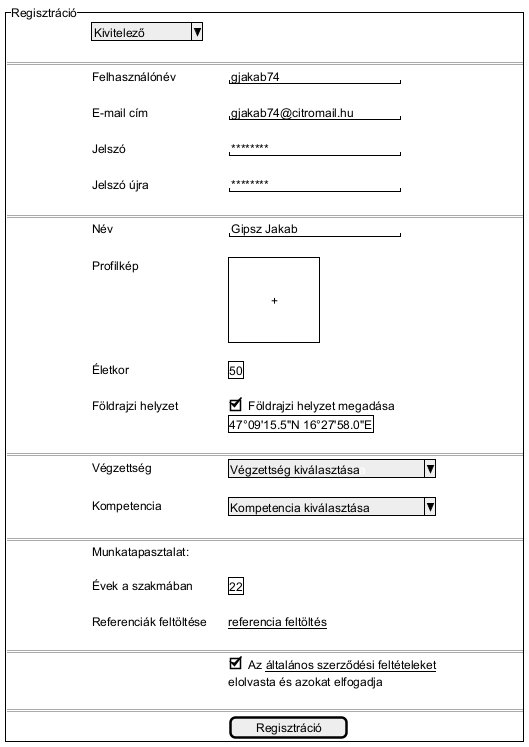
\includegraphics[scale=0.5]{img/regisztracio.png}
	\caption*{Regisztráció}
	\label{fig:reg}
\end{figure}